% !TEX TS-program = pdflatex
% !TEX encoding = ISOLatin2


\documentclass[10pt,a4paper,parskip]{scrbook}
\usepackage[T1]{fontenc}
\usepackage{textcomp}
\usepackage[scaled=.92]{helvet}
\usepackage{courier}
\usepackage{amsmath}
\usepackage{amssymb}
%\usepackage{mathabx}% for circles in tables
\usepackage{pifont}
%\usepackage[varg]{txfonts}
\usepackage{tikz}
\usetikzlibrary{shapes,shadows,arrows,patterns,trees,automata,positioning,snakes}
\usetikzlibrary{decorations.text}
\usetikzlibrary{decorations.fractals}
\usetikzlibrary{decorations.markings}
\usetikzlibrary{decorations.pathmorphing}
\usetikzlibrary{decorations.text}
\usetikzlibrary{decorations.footprints}
\usetikzlibrary{decorations.pathreplacing}
\usetikzlibrary{decorations.shapes}

\usepackage[active,tightpage]{preview}
\PreviewEnvironment{tikzpicture}


\pagestyle{empty}


\begin{document}

%\tikzstyle{every node}=[font=\large]
\tikzstyle{graphnode}=[fill=black!20,circle,inner sep=5pt,draw]
\tikzstyle{emptynode}=[fill=white,circle,inner sep=5pt,draw]
\tikzstyle{sinknode}=[style=graphnode,fill=black!60]
\tikzstyle{descnode}=[draw,rounded corners,node distance=1.7cm,inner sep=7pt,text width=4em,text centered]
\tikzstyle{lowdescnode}=[style=descnode,node distance=1.1cm]
\tikzstyle{level 1}=[level distance=3cm,sibling distance=8cm]
\tikzstyle{level 2}=[level distance=3cm,sibling distance=5cm]
\tikzstyle{level 3}=[level distance=3cm,sibling distance=3cm]



\tikzstyle{junction} = [shape=circle, minimum size=0.5cm, circular drop shadow, text=black, very thick, draw=black!55, top color=white,bottom color=black!20, text width=0.3cm, align=center]

\tikzstyle{big junction} = [shape=circle, minimum size=0.5cm, circular drop shadow, text=black, very thick, draw=black!55, top color=white,bottom color=black!20, text width=2.3cm, align=center]

\tikzstyle{street} = [shape=diamond, minimum size=1cm, draw=black!55, very thick, fill=black!30]
\tikzstyle{dead end} = [outer sep=0,inner sep=0,minimum size=0]


\tikzstyle{street edge} = [draw=black!55, line width=2]

\tikzstyle{routing edge} = [draw=black!55, line width=5]






\begin{tikzpicture}

\node[opacity=0.2] (background_image) at (466.241875pt,331.2375pt) { 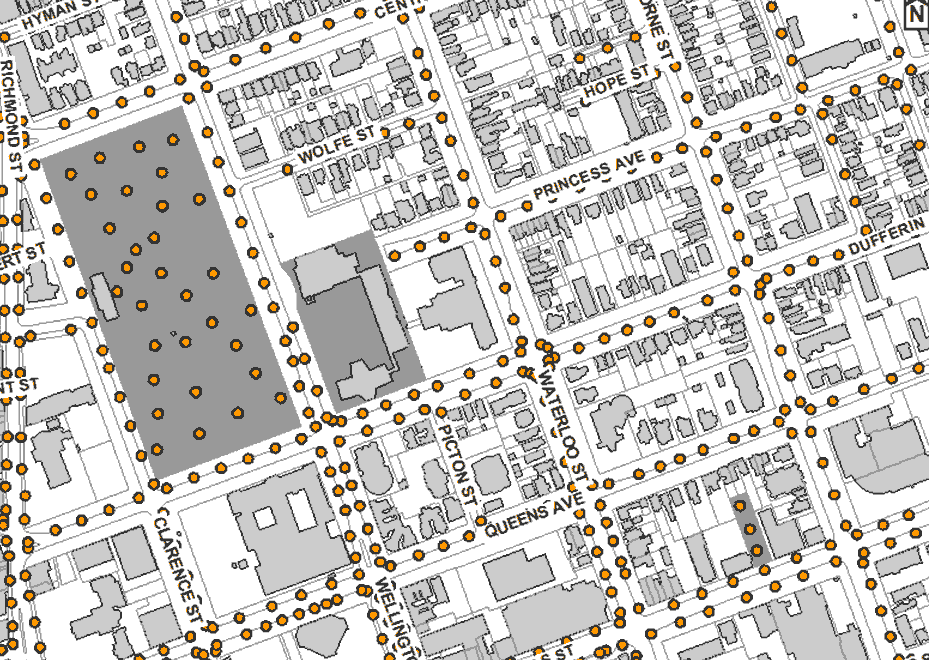
\includegraphics{overlay.png} };

% left bottom right top
  \useasboundingbox  (-0.2,-0.2) rectangle (32.6, 23.2);
%grapgtotikz size: 32.8  23.0


\node (v194) at (5.5,6) [junction] {};
\node (v193) at (0.5,4) [junction] {};
\node (v198) at (0.5,11.5) [junction] {};
\node (v200) at (0.5,18) [junction] {};
\node (v202) at (6.81,20.52) [junction] {};
\node (v300) at (6.476,21.81) [street] {};
\node (v204) at (14.24,23.1) [junction] {};
\node (v333) at (11.62,17.95) [street] {};
\node (v206) at (16.95,15.38) [junction] {};
\node (v208) at (18.81,10.62) [junction] {};
\node (v329) at (0.7619,1.81) [street] {};
\node (v210) at (26.57,13.29) [junction] {};
\node (v314) at (32.24,19.57) [street] {};
\node (v212) at (24.75,18.29) [junction] {};
\node (v312) at (29.48,17.33) [street] {};
\node (v214) at (28.57,19.68) [junction] {};
\node (v306) at (26.68,18.96) [street] {};
\node (v216) at (31.81,20.81) [junction] {};
\node (v309) at (23.05,22.71) [street] {};
\node (v296) at (30.67,14.62) [junction] {};
\node (v219) at (28.33,8.667) [junction] {};
\node (v220) at (20.57,5.714) [junction] {};
\node (v316) at (30.33,9.476) [street] {};
\node (v222) at (13,3) [junction] {};
\node (v326) at (10,1.81) [street] {};
\node (v224) at (11.33,7.905) [junction] {};
\node (v226) at (8,16.5) [junction] {};
\node (v228) at (15.52,19.24) [junction] {};
\node (v230) at (22.43,1.048) [junction] {};
\node (v231) at (30.05,3.857) [junction] {};
\node (v323) at (14.67,9.238) [street] {};
\node (v233) at (27.14,2.762) [junction] {};
\node (v322) at (22.33,11.9) [street] {};
\node (v235) at (7.19,0.619) [junction] {};
\node (v236) at (23.39,21.96) [junction] {};
\node (v334) at (10.33,21.81) [street] {};
\node (v305) at (20.81,16.95) [street] {};
\node (v313) at (31.33,22.1) [street] {};
\node (v311) at (27.95,21.52) [street] {};
\node (v315) at (27.43,10.95) [street] {};
\node (v320) at (21.43,3.429) [street] {};
\node (v328) at (6.238,0.1905) [street] {};
\node (v327) at (6.286,3.524) [street] {};
\node (v252) at (27.38,23.19) [dead end] {};
\node (v253) at (20.43,21.14) [dead end] {};
\node (v254) at (6.048,22.86) [dead end] {};
\node (v255) at (0.09524,22.05) [dead end] {};
\node (v447) at (1.429,0.2381) [dead end] {};
\node (v257) at (13.71,0.1429) [dead end] {};
\node (v450) at (0.2857,0.2857) [dead end] {};
\node (v259) at (19.95,0.04762) [street] {};
\node (v260) at (30.95,23.24) [dead end] {};
\node (v261) at (32.76,18.14) [dead end] {};
\node (v262) at (32.43,10.24) [dead end] {};
\node (v263) at (31.81,0.1429) [dead end] {};
\node (v264) at (32.19,4.762) [street] {};
\node (v307) at (25.62,15.76) [street] {};
\node (v308) at (23.9,20.38) [street] {};
\node (v310) at (21.95,21.57) [street] {};
\node (v317) at (29.19,6.095) [street] {};
\node (v319) at (24.76,1.952) [street] {};
\node (v318) at (30.95,1.952) [street] {};
\node (v325) at (13.38,1.619) [street] {};
\node (v324) at (12.1,5.667) [street] {};
\node (v301) at (0.2857,20.24) [street] {};
\node (v304) at (15.33,14.86) [street] {};
\node (v303) at (17.71,13.19) [street] {};
\node (v281) at (26.1,5.524) [dead end] {};
\node (v321) at (19.62,8.19) [street] {};
\node (v283) at (13.71,14.33) [dead end] {};
\node (v331) at (0.5238,14.86) [street] {};
\node (v330) at (0.5714,8) [street] {};
\node (v373) at (16.57,4.333) [street] {};
\node (v379) at (24,7) [street] {};
\node (v388) at (28.57,3.238) [street] {};
\node (v391) at (26.62,4.238) [street] {};
\node (v402) at (28.48,13.9) [street] {};
\node (v407) at (30.1,20.19) [street] {};
\node (v442) at (16.24,17.33) [street] {};
\node (v439) at (14.81,21.24) [street] {};
\node (v458) at (3,12) [junction] {};
\node (v460) at (1.7,11.7) [street] {};
\node (v482) at (5.5,14) [big junction] {};
\node (v491) at (3,5) [street] {};

\draw[street edge] (v323) to (v208);
\draw[street edge] (v208) to (v321);
\draw[street edge] (v321) to (v220);
\draw[street edge] (v193) to (v330);
\draw[street edge] (v200) to (v301);
\draw[street edge] (v204) to (v334);
\draw[street edge] (v334) to (v202);
\draw[street edge] (v193) to (v491);
\draw[street edge] (v300) to (v254);
\draw[street edge] (v224) to (v323);
\draw[street edge] (v200) to (v331);
\draw[street edge] (v301) to (v255);
\draw[street edge] (v324) to (v222);
\draw[street edge] (v331) to (v198);
\draw[street edge] (v198) to (v460);
\draw[street edge] (v329) to (v193);
\draw[street edge] (v202) to (v300);
\draw[street edge] (v447) to (v329);
\draw[street edge] (v198) to (v330);
\draw[street edge] (v329) to (v450);
\draw[street edge] (v328) to (v235);
\draw[street edge] (v235) to (v327);
\draw[street edge] (v327) to (v194);
\draw[street edge] (v224) to (v324);
\draw[street edge] (v222) to (v326);
\draw[street edge] (v326) to (v235);
\draw[street edge] (v257) to (v325);
\draw[street edge] (v325) to (v222);
\draw[street edge] (v220) to (v373);
\draw[street edge] (v373) to (v222);
\draw[street edge] (v230) to (v259);
\draw[street edge] (v230) to (v320);
\draw[street edge] (v320) to (v220);
\draw[street edge] (v220) to (v379);
\draw[street edge] (v379) to (v219);
\draw[street edge] (v219) to (v317);
\draw[street edge] (v317) to (v231);
\draw[street edge] (v231) to (v264);
\draw[street edge] (v231) to (v318);
\draw[street edge] (v318) to (v263);
\draw[street edge] (v231) to (v388);
\draw[street edge] (v388) to (v233);
\draw[street edge] (v281) to (v391);
\draw[street edge] (v391) to (v233);
\draw[street edge] (v233) to (v319);
\draw[street edge] (v319) to (v230);
\draw[street edge] (v208) to (v322);
\draw[street edge] (v210) to (v322);
\draw[street edge] (v210) to (v315);
\draw[street edge] (v315) to (v219);
\draw[street edge] (v219) to (v316);
\draw[street edge] (v316) to (v262);
\draw[street edge] (v210) to (v402);
\draw[street edge] (v402) to (v296);
\draw[street edge] (v296) to (v312);
\draw[street edge] (v312) to (v214);
\draw[street edge] (v214) to (v407);
\draw[street edge] (v407) to (v216);
\draw[street edge] (v216) to (v314);
\draw[street edge] (v261) to (v314);
\draw[street edge] (v216) to (v313);
\draw[street edge] (v313) to (v260);
\draw[street edge] (v311) to (v252);
\draw[street edge] (v311) to (v214);
\draw[street edge] (v214) to (v306);
\draw[street edge] (v306) to (v212);
\draw[street edge] (v212) to (v307);
\draw[street edge] (v307) to (v210);
\draw[street edge] (v212) to (v305);
\draw[street edge] (v305) to (v206);
\draw[street edge] (v206) to (v304);
\draw[street edge] (v304) to (v283);
\draw[street edge] (v206) to (v303);
\draw[street edge] (v208) to (v303);
\draw[street edge] (v212) to (v308);
\draw[street edge] (v308) to (v236);
\draw[street edge] (v236) to (v309);
\draw[street edge] (v236) to (v310);
\draw[street edge] (v310) to (v253);
\draw[street edge] (v442) to (v228);
\draw[street edge] (v442) to (v206);
\draw[street edge] (v228) to (v333);
\draw[street edge] (v333) to (v226);
\draw[street edge] (v202) to (v334);
\draw[street edge] (v439) to (v204);
\draw[street edge] (v439) to (v228);
\draw[street edge] (v460) to (v458);
\draw[routing edge] (v458) to (v482);
\draw[routing edge] (v482) to (v226);
\draw[routing edge] (v202) to (v482);
\draw[routing edge] (v200) to (v482);
\draw[routing edge] (v194) to (v482);
\draw[routing edge] (v224) to (v482);
\draw[street edge] (v491) to (v194);






%add border
\foreach \border in {0.2}
  \useasboundingbox (current bounding box.south west)+(-\border,-\border) rectangle (current bounding box.north east)+(\border,\border);


\end{tikzpicture}



\end{document}

